% tikz-bidang-diagonal-balok.tex
\documentclass[tikz]{standalone}
\usepackage{amsmath}
\usetikzlibrary{}
\definecolor{bgpage}{HTML}{171D2B}
\definecolor{aksen}{HTML}{F7B538}
\begin{document}
\pagecolor{bgpage}
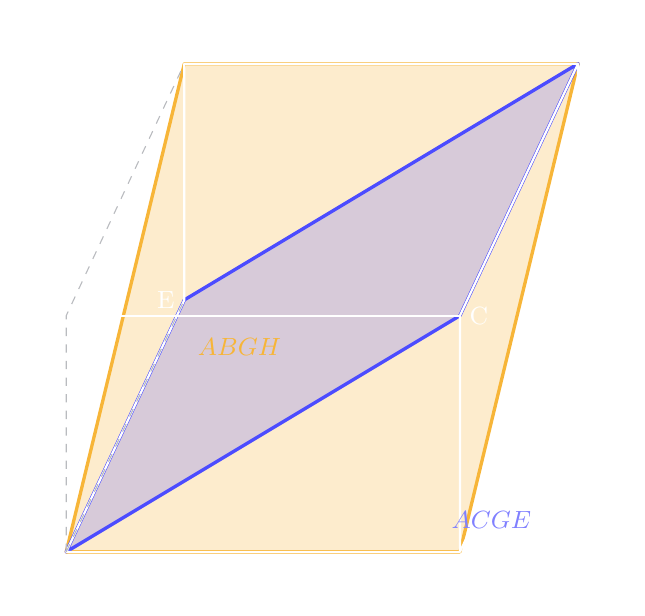
\begin{tikzpicture}[
  scale=1.0,
  line join=round,
  text=white,
  visible/.style={thick, draw=white},
  hidden/.style={thin, dashed, draw=white!70!bgpage},
  diagplane/.style={draw=aksen, very thick},
]
  \def\p{5} \def\l{3} \def\t{3.2}
  \def\dx{1.5} \def\dy{1.1}

  \coordinate (A) at (0,0);
  \coordinate (B) at (\p,0);
  \coordinate (C) at (\p,\l);
  \coordinate (D) at (0,\l);
  \coordinate (E) at (\dx,\t);
  \coordinate (F) at (\p+\dx,\t);
  \coordinate (G) at (\p+\dx,\l+\t);
  \coordinate (H) at (\dx,\l+\t);

  % bidang diagonal 1: ABGH (aksen kuning, semi transparan)
  \fill[aksen, opacity=0.25] (A) -- (B) -- (G) -- (H) -- cycle;
  \draw[diagplane] (A) -- (B) -- (G) -- (H) -- cycle;

  % bidang diagonal 2: ACGE (biru, semi transparan)
  \fill[blue!60, opacity=0.25] (A) -- (C) -- (G) -- (E) -- cycle;
  \draw[blue!70, very thick] (A) -- (C) -- (G) -- (E) -- cycle;

  % rusuk terlihat
  \draw[visible] (A) -- (B) -- (F) -- (G) -- (H) -- (E) -- cycle;
  \draw[visible] (B) -- (C) -- (G);
  \draw[visible] (D) -- (C);

  % rusuk tersembunyi
  \draw[hidden] (A) -- (D) -- (H);
  \draw[hidden] (A) -- (E);

  \foreach \pt/\pos in {A/below left, B/below right, C/right, D/above left,
                        E/left, F/above right, G/above right, H/above left}
    \node[\pos, font=\small, text=white] at (\pt) {\pt};

  \node[font=\small, text=aksen] at (2.2,2.6) {$ABGH$};
  \node[font=\small, text=blue!50] at (5.4,0.4) {$ACGE$};
\end{tikzpicture}
\end{document}
